\documentclass[11pt]{article}

\usepackage[utf8]{inputenc}
\usepackage[margin=1in]{geometry} 
\usepackage{amsmath,amsthm,amssymb,graphicx,mathtools,tikz,hyperref,multicol,cancel,enumitem,booktabs,float,pgfplots,multirow,mathrsfs,textcomp,gensymb,soul,changepage,threeparttable}
%\usepackage[table]{xcolor}
\usepackage[T1]{fontenc}
\usepackage[italian]{babel}
\usepackage{hyphenat}
\hyphenation{mate-mati-ca recu-perare}
\usetikzlibrary{positioning}
\pgfplotsset{compat=1.14}

\newcommand{\n}{\mathbb{N}}
\newcommand{\z}{\mathbb{Z}}
\newcommand{\q}{\mathbb{Q}}
\newcommand{\cx}{\mathbb{C}}
\newcommand{\real}{\mathbb{R}}
\newcommand{\field}{\mathbb{F}}
\newcommand{\ita}[1]{\textit{#1}}
\newcommand{\com}[2]{#1\backslash#2}
\newcommand{\oneton}{\{1,2,3,...,n\}}
\newcommand{\idea}[1]{\begin{gather*}#1\end{gather*}}
\newcommand{\ef}{\ita{f} }
\newcommand{\eff}{\ita{f}}
\newcommand{\proofs}[1]{\begin{proof}#1\end{proof}}
\newcommand{\inv}[1]{#1^{-1}}
\newcommand{\setb}[1]{\{#1\}}
\newcommand{\en}{\ita{n }}
\newcommand{\vbrack}[1]{\langle #1\rangle}
\newcommand{\qRa}{\quad \Rightarrow \quad}
\newcommand{\smaca}[1]{\textbf{\textsc{#1}}}

\newenvironment{theorem}[2][Teorema]{\begin{trivlist}
\item[\hskip \labelsep {\bfseries #1}\hskip \labelsep {\bfseries #2.}]}{\end{trivlist}}
\newenvironment{lemma}[2][Lemma]{\begin{trivlist}
\item[\hskip \labelsep {\bfseries #1}\hskip \labelsep {\bfseries #2.}]}{\end{trivlist}}
\newenvironment{exercise}[2][Esercizio]{\begin{trivlist}
\item[\hskip \labelsep {\bfseries #1}\hskip \labelsep {\bfseries #2.}]}{\end{trivlist}}
\newenvironment{proposition}[2][Proposizione]{\begin{trivlist}
\item[\hskip \labelsep {\bfseries #1}\hskip \labelsep {\bfseries #2.}]}{\end{trivlist}}
\newenvironment{corollary}[2][Corollario]{\begin{trivlist}
\item[\hskip \labelsep {\bfseries #1}\hskip \labelsep {\bfseries #2.}]}{\end{trivlist}}

\hypersetup {
    colorlinks,
    linkcolor=blue
}

\graphicspath{{img/}}

\begin{document}
\setlength{\parindent}{0pt}
\title{\vspace{-4em}{\large Laboratorio di Meccanica e Termodinamica} \\
    Relazione di Laboratorio}
\author{Gerardo Selce, Maurizio Liguori, Emanuela Galluccio, Francesco Messano}
\date{29/10/2024}
\maketitle

\vspace{-2em}\par\noindent\rule{\textwidth}{0.4pt}
\begin{center}
    {\Large\sc Misura di una variabile casuale} 
\end{center}
\par\noindent\rule{\textwidth}{0.4pt}

\section{Scopo dell'esperienza}
Assegnato un lotto di 250 rondelle dello stesso tipo, si vuole misurarne il diametro attraverso uno strumento di precisione. I dati raccolti possono essere descritti da una variabile casuale di cui si intende studiare le principali proprietà statistiche.

\begin{figure}[ht]
  \centering
  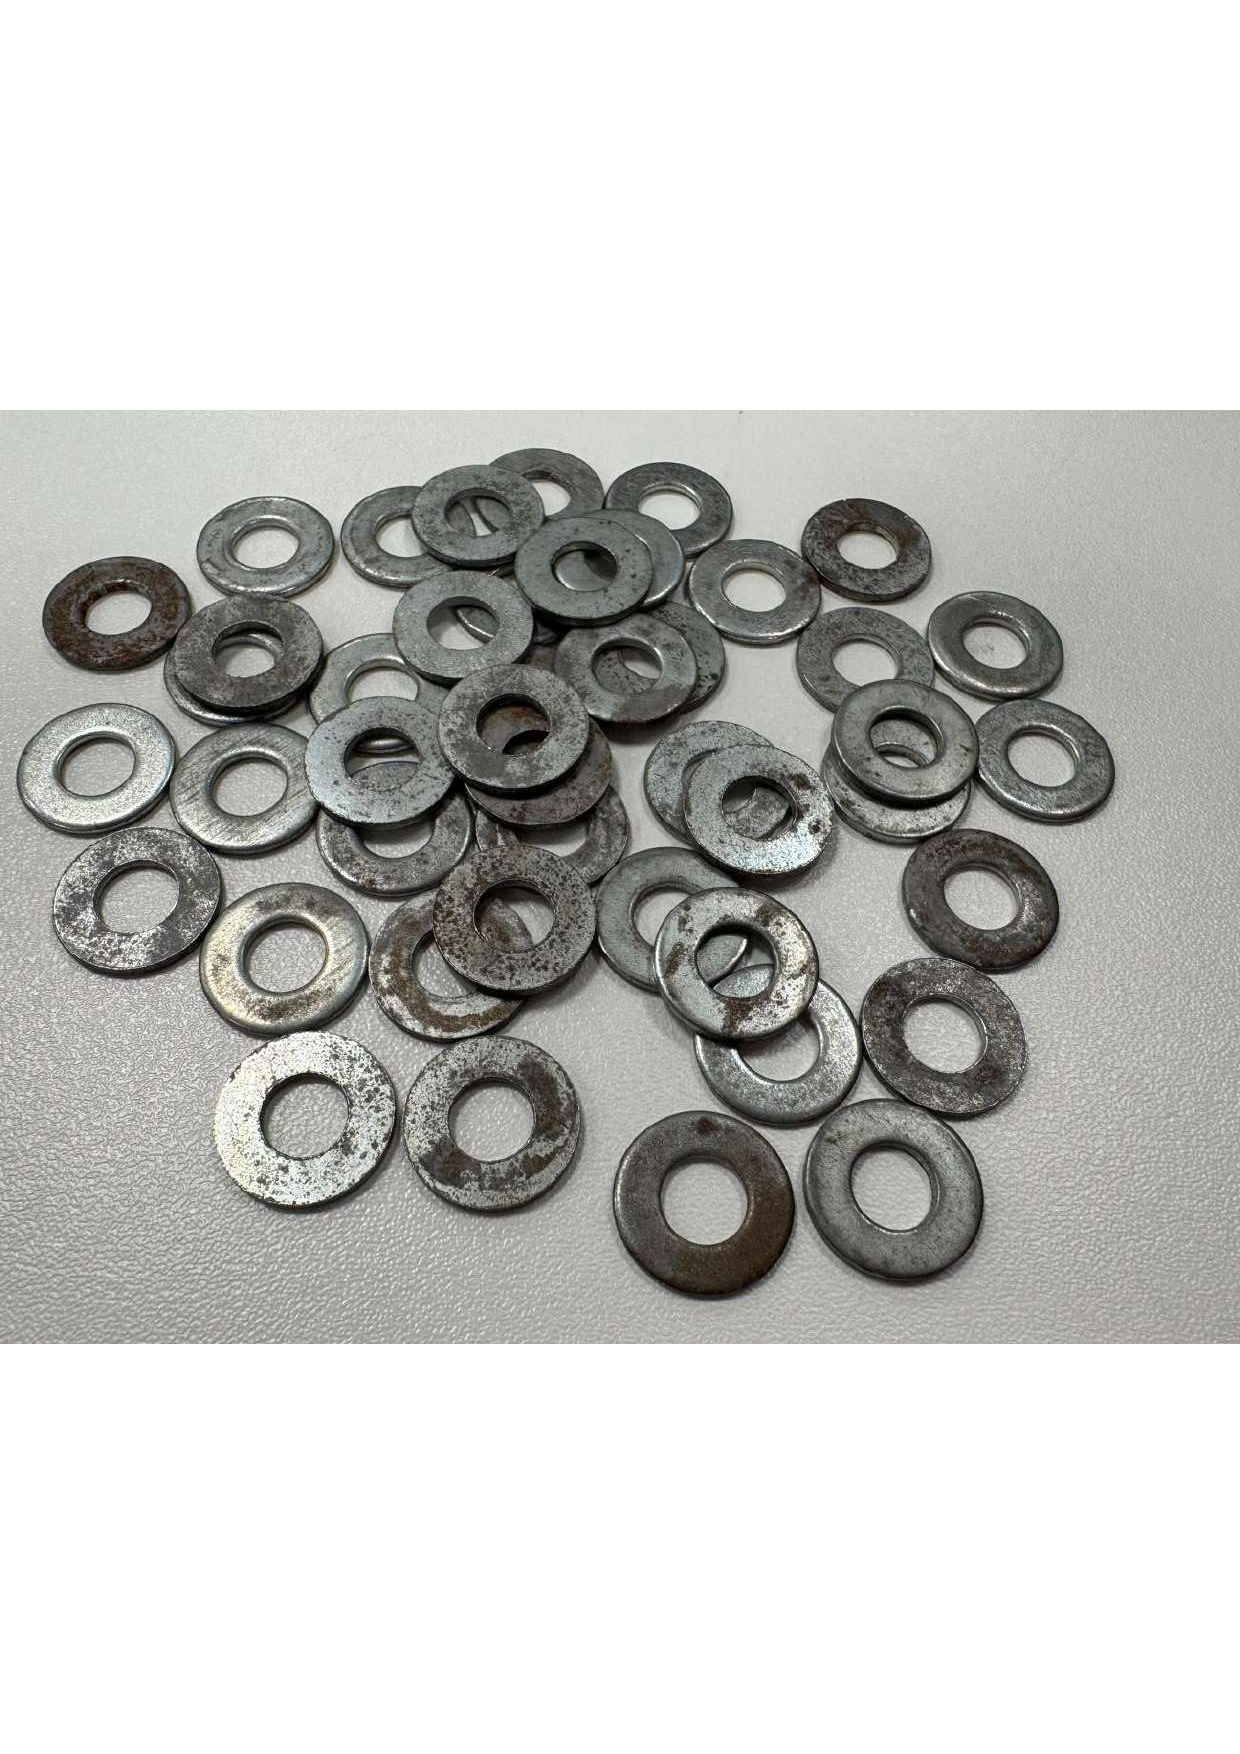
\includegraphics[width=0.35\textwidth]{Immagine WhatsApp 2024-11-01 ore 17.29.35_0368a3ac.pdf}
  \caption{Rondelle utilizzate in laboratorio}
\end{figure}

\section{Richiami teorici}
Quando da una serie di misurazioni dirette di una grandezza fisica (con lo stesso strumento, nelle stesse condizioni e seguendo la stessa procedura) si ottengono risultati leggermente diversi e non prevedibili, la misura si dice affetta da errori casuali. Essi nascono dall'impossibilità di riprodurre esattamente le stesse condizioni sperimentali. \\ \\ Ad ogni misurazione infatti, intervengono varizioni minime, ma incontrollabili e imprevedibili di tali condizioni, che producono leggere variazioni casuali nei risultati (se la misurazione è sufficientemente precisa). \\ \\ Gli errori casuali sono osservabili solo se lo strumento è sufficientemente sensibile da generare errori maggiori dell'errore di sensibilità. Se così non fosse, i risultati delle diverse misurazioni coinciderebbero e l'errore sarebbe sempre quello strumentale. Per gestire ed interpretare correttamente queste fluttuazioni, è necessario ricorrere a metodi statistici.
\\ \\
Una distribuzione di dati può essere descritta attraverso indici di posizione e di dispersione. Gli indici di posizione sono misure statistiche che descrivono valori rappresentativi dell'intera distribuzione di dati. I più comuni sono i seguenti:
\begin{itemize}
    \item \textbf{Media:} Considerato un campione di N misure $\{x_0, x_1, ..., x_N\}$ indichiamo media aritmetica il valore $$\overline{x}=\frac{\displaystyle\sum_{i=1}^{N}x_i}{N}$$
    \item \textbf{Mediana:} Indichiamo mediana il valore che divide in due parti uguali l'insieme campione ordinato.
    \item \textbf{Moda:} Indichiamo moda il valore che ha frequenza più alta nell'insieme campione.
\end{itemize}
Gli indici di dispersione invece misurano la variabilità dei dati. I più comuni sono i seguenti:
\begin{itemize}
    \item \textbf{Dispersione:} Indichiamo dispersione la differenza $$d=max(x_i) - min(x_i)$$
    \item \textbf{Scarto quadratico medio:} Indichiamo scarto quadratico medio il valore $$\xi_q=\sqrt{\frac{\displaystyle\sum_{i=1}^{N}(x_i - \overline{x})^2}{N}}$$ Lo scarto quadratico medio fornisce una misura della concentrazione dei dati intorno alla media aritmentica.
\end{itemize}

\subsection{Istogramma delle Frequenze}

Per ottenere una rappresentazione visiva dei dati raccolti si ricorre ad un istogramma delle frequenze. Considerato un campione di $N$ misure $\{x_0, x_1, ..., x_N\}$, si considera l'intervallo: $$[min(x_i), max(x_i)]$$
Consideriamo successivamente una partizione dell'intervallo in un numero $k$ di sottointervalli, compatibile con la seguente condizione empirica: $$k\leq\sqrt{N}$$ Sull'asse orizzontale rappresentiamo l'intervallo partizionato, mentre su quello verticale riportiamo le frequenze assolute, relative o di densità dei valori ottenuti.
\\
\begin{table}[H]
\centering
\resizebox{\columnwidth}{!}{
\begin{tabular}{|l|c|l|c|}
\hline

Frequenza assoluta & Frequenza relativa & Densità di frequenza \\ \hline
$m_k$ & $f_k=\frac{m_k}{N}$ & $h_k=\frac{f_k}{\Delta_k}$, $\Delta_k=a_k-a_{k-1}$ \\ \hline
\end{tabular}
}
\end{table}


\section{Descrizione dell'apparato sperimentale}
Le misurazioni dei diametri sono state ottenute con un micrometro Palmer. Il micrometro Palmer, o calibro micrometrico, è uno strumento di misura di alta precisione, usato per misurare piccoli spessori e diametri con accuratezza fino al centesimo o millesimo di millimetro. È costituito da una vite micrometrica e un tamburo graduato, che permettono di misurare con precisione lo spostamento dell'asta mobile verso un cilindro fisso, con cui l'oggetto da misurare viene messo a contatto. Alcuni modelli includono un cricchetto per applicare una pressione costante, assicurando misurazioni più affidabili.
\\\\
Il micrometro utilizzato per l'esperimento presenta le seguenti caratteristiche:
\\ \textbf{Risoluzione:} $0.01mm$
\\ \textbf{Sensibilità:} $100\ div/mm$
\begin{figure}[H]
  \centering
  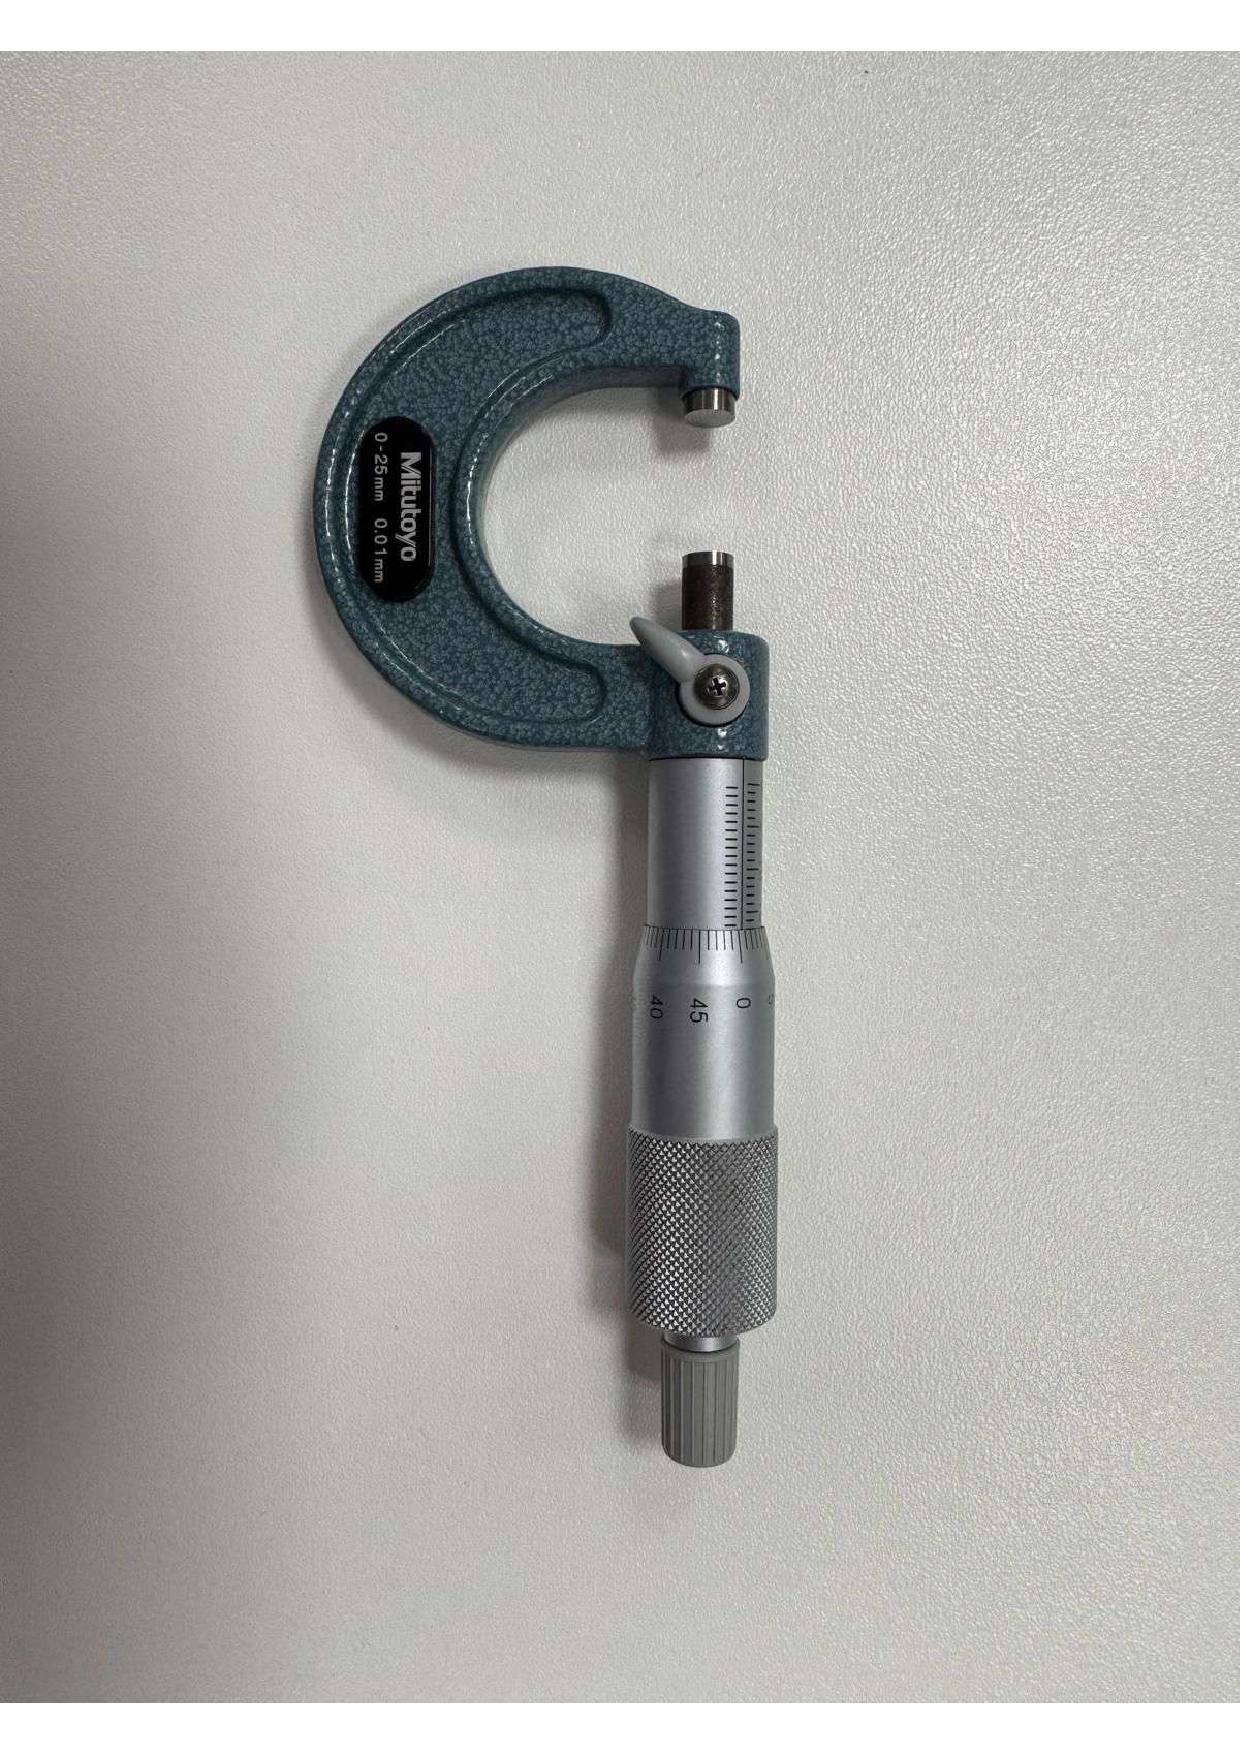
\includegraphics[width=0.35\textwidth]{micrometro.pdf}
  \caption{Micrometro Palmer}
\end{figure}


\section{Descrizione dei dati sperimentali}
\begin{table}[H]
\centering
\begin{tabular}{|c|c|}
\hline
\textbf{Valore ($mm$)} & \textbf{Frequenza Assoluta} \\
\hline
17.665 & 22 \\
17.695 & 21 \\
17.670 & 20 \\
17.675 & 17 \\
17.665 & 16 \\
17.705 & 15 \\
17.685 & 14 \\
17.660 & 13 \\
17.690 & 10 \\
17.680 & 9 \\
17.650 & 9 \\
17.645 & 9 \\
17.730 & 9 \\
17.715 & 8 \\
17.750 & 7 \\
17.720 & 7 \\
17.745 & 6 \\
17.700 & 6 \\
17.725 & 6 \\
17.710 & 5 \\
17.630 & 4 \\
17.625 & 3 \\
17.635 & 3 \\
17.735 & 3 \\
17.755 & 3 \\
17.640 & 3 \\
17.610 & 1 \\
17.585 & 1 \\
17.615 & 1 \\
17.740 & 1 \\
\hline
\end{tabular}
\caption{Tabella delle frequenze assolute dei valori}
\label{tab:frequenze_assolute}
\end{table}

I dati raccolti nella Teblla 1 sono riportati su un istogramma normalizzato. 

\begin{figure}[H]
  \centering
  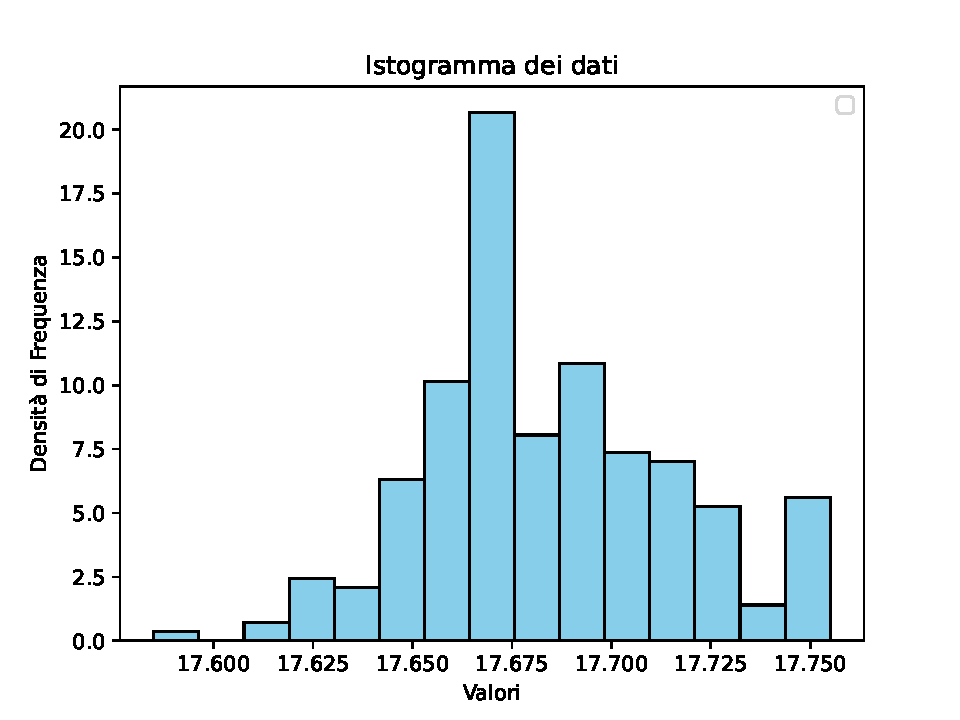
\includegraphics[width=1\textwidth]{istogramma.pdf}
  \caption{$N=250$,\
   $k=15$,\
   $[17.585, 17.755]\ mm$,\
   $\Delta\approx0.011\ mm$}
\end{figure}

\section{Analisi dei dati sperimentali}
L'istogramma normalizzato e gli indici di posizione e dispersione sono stati ottenuti tramite uno script scritto in python.
\\
$$Media=17.681\ mm$$ 
$$Mediana=17.680\ mm$$ 
$$Moda=17.685\ mm$$ 
$$Deviazione\ Standard=0.032\ mm$$
\\
Di seguito sono riportate le frequenze relative entro $k$ deviazioni standard dalla media: $$[\overline{x}-k\xi_q,\ \overline{x}+k\xi_q],\ k\in[1,2,3]$$

\begin{itemize}
    \item $k=1 \ \Rightarrow \ 59\%$
    \item $k=2 \ \Rightarrow \ 88\%$
    \item $k=3 \ \Rightarrow \ 99\%$
\end{itemize}

\section{Conclusioni}
La media e la mediana risultano pressoché identiche, pari rispettivamente a 17,681 mm e 17,680 mm, mentre la moda si discosta leggermente, attestandosi a 17,685 mm. La deviazione standard, pari a 0,032 mm, indica un’elevata precisione delle misurazioni, confermata dall’analisi dell’intervallo di dispersione: circa il 59\% dei valori si colloca entro una deviazione standard dalla media, l’88\% entro due e il 99\% entro tre. I risultati sono comptibili con una distribuzione standard dell'errore.

\end{document}